\section{Background and Motivation}
\label{sec:background}

\subsection{Latency-Critical Onboard Perception}
\label{sec:bg:robotics}

Robotic perception runs inside an online sensing-to-action
loop~\cite{percsurvey,navsurvey}. Optical flow supplies motion estimates and
depth supplies obstacle geometry for navigation~\cite{nanoflownet,fastdepth},
segmentation supplies scene state for planning~\cite{bisenet}, and object pose
and grasp proposals guide manipulation~\cite{densefusion,contactgraspnet}. In
each case the inference output feeds a downstream component whose next decision
depends on the freshness of that estimate~\cite{pampc,perclatency}. Because
freshness is set by latency, a lower perception latency is always preferable:
where a task imposes a latency budget, a lower latency makes that budget easier
to meet; where none is fixed, it still lets the controller react to the
environment sooner~\cite{eventavoid,dronerace}. We therefore target latency
minimization rather than a preset deadline. Offloading to remote compute could
add capacity but is bounded by communication delay and
connectivity~\cite{cloudrobotics}, so we close the loop onboard under a limited
power and compute budget~\cite{onboardsensing}, minimizing end-to-end perception
latency on the target device.

One line of work is targeted to lower this latency by computing only the active region of each
frame, delivered as a spatial mask. The mask derives from event-camera
increments~\cite{asyncsparse,evconv}, temporal residuals between video
frames~\cite{cbinfer,skipconv,deltacnn}, or learned input-dependent
gates~\cite{sact,sai,dgnet,dynconv}. These sources differ in sensing modality
and policy, but all expose the same spatial sparsity on a dense 2D feature grid
for the convolution operator to exploit.

\subsection{Masked Convolution}
\label{sec:bg:masked}

Masked convolution keeps the dense tensors and arithmetic of a dense convolution
and restricts only which output coordinates it evaluates. It operates on an input
feature tensor $\mathbf{x}\in\mathbb{R}^{H_{in}\times W_{in}\times C_{in}}$, a
weight tensor $\mathbf{w}\in\mathbb{R}^{k\times k\times C_{in}\times C_{out}}$ of
kernel size $k$, and an output
$\mathbf{y}\in\mathbb{R}^{H_{out}\times W_{out}\times C_{out}}$ on a coordinate
grid $\mathcal{G}=\{1,\ldots,H_{out}W_{out}\}$, where each coordinate $p$ has a
$k\times k$ receptive field $\mathcal{N}(p)$ in $\mathbf{x}$. An upstream policy
marks the coordinates to compute in an output mask
$M_{out}\in\{0,1\}^{H_{out}\times W_{out}}$. Spatial gating predicts $M_{out}$
directly; event and temporal policies instead supply an input mask
$M_{in}\in\{0,1\}^{H_{in}\times W_{in}}$ whose active positions propagate their
influence along the receptive field, so $p$ stays active whenever any input in
$\mathcal{N}(p)$ is active,
\begin{equation}
  M_{out}[p] =
  \begin{cases}
    1, & \exists\, r\in\mathcal{N}(p)\ \text{s.t.}\ M_{in}[r]=1,\\
    0, & \text{otherwise.}
  \end{cases}
  \label{eq:mask}
\end{equation}
$M_{out}$ thus fixes which positions of $\mathbf{y}$ the operator updates, each
by aggregating $\mathbf{x}$ over $\mathcal{N}(p)$ with the weights $\mathbf{w}$.
The active ratio $\alpha = \|M_{out}\|_0 / |\mathcal{G}|$, the active fraction of
the grid, is the intrinsic sparsity the policy exposes.

An execution path realizes this mask over a compute set $\mathcal{C}$ bounded by
$\{p : M_{out}[p]=1\}\subseteq\mathcal{C}\subseteq\mathcal{G}$; for each
$p\in\mathcal{C}$ it computes
\begin{equation}
  \mathbf{y}[p] = \sum_{i=1}^{k^2}
  \mathbf{w}_i\,\mathbf{x}[\mathcal{N}_i(p)],
  \label{eq:conv}
\end{equation}
where $\mathcal{N}_i(p)$ is the $i$-th position in $\mathcal{N}(p)$ and
$\mathbf{w}_i\in\mathbb{R}^{C_{in}\times C_{out}}$ the corresponding weight
slice. The path must compute every active coordinate to avoid dropping a
requested output but may also compute inactive ones; dense convolution is the
extreme $\mathcal{C}=\mathcal{G}$. The policy alone fixes the accuracy and the
required work, while the choice of $\mathcal{C}$ is determined by the path.

\subsection{The Sparsity-to-Latency Gap}
\label{sec:bg:gap}

Existing systems execute a mask along one of two paths. \emph{Tile
skipping}~\cite{sbnet,skipconv,evconv} inherits the dense pipeline's tile-based
computation, skipping a tile only when all its coordinates are inactive and
otherwise computing the whole tile; DeltaCNN~\cite{deltacnn} fuses a selective
path into the kernel, taken when a tile is estimated to be mostly empty, cutting
wasted work while degrading throughput. \emph{Gather-scatter}~\cite{sai,dgnet}
instead extracts exactly the active coordinates, computes, and scatters them
back, removing the inactive arithmetic but adding extraction, irregular access,
and writeback overhead; DynConv~\cite{dynconv} adopts a model structure suited to
gather-scatter, where one gather feeds several consecutive layers before a single
scatter, amortizing that overhead.

We measure each path by two quantities. Its useful-compute ratio is the
fraction of computed coordinates that are active,
\begin{equation}
  \eta = \frac{\|M_{out}\|_0}{|\mathcal{C}|} \le 1.
  \label{eq:useful-ratio}
\end{equation}
Its throughput is the rate at which it processes issued FLOPs,
\begin{equation}
  T = \frac{2\,|\mathcal{C}|\,k^2 C_{in} C_{out}}{t},
  \label{eq:throughput}
\end{equation}
where $t$ is the per-frame latency and the leading factor of 2 counts each
multiply-accumulate as two FLOPs. For the required
$2\,\|M_{out}\|_0\,k^2 C_{in} C_{out}$ FLOPs, latency is set by the \textbf{effective
throughput} $T_{\mathrm{eff}} = \eta T$, the rate at which a path computes needed
outputs.

Figure~\ref{fig:gap} traces this on Jetson AGX Orin for the sparsest workload in our evaluation.
The policy marks 84.4\% of the convolution work unnecessary, and the sparse paths
discard it with negligible accuracy loss, so the remaining work sets a 9.6\,ms
latency floor (Fig.~\ref{fig:gap}a, dashed). Neither path approaches it: tile
skipping (DeltaCNN~\cite{deltacnn}) reaches 36.6\,ms, still 3.8$\times$ the floor, and gather-scatter, the
path DynConv is built around, runs at 194\,ms, far slower than dense convolution
itself. That is due to their low effective throughput from different causes. Tile skipping holds
throughput near half of dense but at a useful-compute ratio of only 0.49;
gather-scatter lifts the useful-compute ratio to one, yet extraction and data
movement collapse its throughput to 5\% of dense (Fig.~\ref{fig:gap}b). Neither
path efficiently converts the GPU's capability into effective throughput.

\begin{figure}[t]
  \centering
  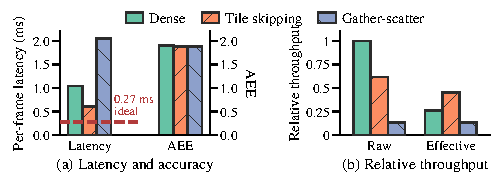
\includegraphics[width=\columnwidth]{figures/gap.pdf}
  \caption{Statistics of DynConv~\cite{dynconv}, a pose estimator
  with learned spatial gating, on the MPII human-pose dataset~\cite{mpii} and
  Jetson AGX Orin, comparing the native cuDNN path (Dense) against the two
  sparse paths.
  (a)~End-to-end average per-frame latency (left axis; the dashed line marks the
  dense latency scaled by the active ratio aggregated across layers) and PCKh
  accuracy (right axis; keypoints localized within half the head size). The
  sparse paths apply the same mask, so their accuracy coincides. (b)~Raw
  throughput $T$ and effective throughput $T_{\mathrm{eff}}$, aggregated across
  the model's convolution layers. The dense useful-compute ratio implies the
  active ratio set by DynConv's spatial gating ($\alpha\approx15.6\%$).}
  \label{fig:gap}
\end{figure}

\subsection{Relation to 3D Sparse Convolution}
\label{sec:bg:3d}

SpConv~v2 and TorchSparse++ target point clouds that are sparse by
representation, building coordinate maps over irregular voxel
coordinates~\cite{spconv2,torchsparsepp}. Our setting instead keeps dense 2D
tensors under a changing spatial mask, where the challenge is to skip inactive
outputs without turning a regular image-grid pipeline into an irregular one. We
therefore treat 3D sparse convolution as related infrastructure rather than a
primary baseline.
